\documentclass[11pt,a4paper]{article}

% ============================================================================
% Packages
% ============================================================================
\usepackage[utf8]{inputenc}
\usepackage[T1]{fontenc}
\usepackage{amsmath,amssymb,amsthm}
\usepackage{graphicx}
\usepackage{xcolor}
\usepackage{booktabs}
\usepackage{multirow}
\usepackage{subcaption}
\usepackage{tikz}
\usetikzlibrary{shapes.geometric, arrows.meta, positioning, calc, fit, backgrounds, decorations.pathreplacing, patterns}
\usepackage{pgfplots}
\pgfplotsset{compat=1.17}
\usepackage{hyperref}
\usepackage{cleveref}
\usepackage{algorithm}
\usepackage{algpseudocode}
\usepackage{natbib}
\usepackage{geometry}
\geometry{margin=2.5cm}

% ============================================================================
% Theorem environments
% ============================================================================
\theoremstyle{definition}
\newtheorem{definition}{Definition}[section]
\newtheorem{proposition}{Proposition}[section]
\newtheorem{remark}{Remark}[section]

% ============================================================================
% Title and authors
% ============================================================================
% Alternative, more influential title:
% \title{Adaptivity is All You Need: Why Dynamic Topology Improves Model Performance}
\title{\textbf{Static is a Dead End:}\\[0.3em]
\Large Dynamic Topology as the Fundamental Principle of Neural Efficiency\\[0.2em]
\large From Edge Classifiers to Large Language Models}

\author{
Bentley Yusen Lin$^{1}$ \and William Dah-yom Lim$^{1}$ \and Dave Hsulun Tsai$^{1}$ \and Shawn Zengxiang Li$^{1}$\\[0.5em]
\normalsize $^{1}$Safeware Technologies Inc., Ltd.\\[0.2em]
\normalsize \texttt{Bentley@safeware.com.tw}, \texttt{Dave.Tsai@safeware.com.tw},\\
\normalsize \texttt{William.Lim@safeware.com.tw}, \texttt{Shawn.Li@safeware.com.tw}
}

\date{}

\begin{document}

\maketitle

% ============================================================================
\begin{abstract}
We challenge the 40-year-old foundational assumption of deep learning: that neural architecture, once fixed, remains static. We show this assumption is the root cause of brittleness and inefficiency, and propose to abandon it entirely---introducing ASSTF, a framework that sculpts neural topology continuously. We analyze the Adaptive State-Space Transfer Function (ASSTF), a neuron-level mechanism that augments a standard affine layer with a gated, low-rank structural branch. Because the original core transformation remains intact, ASSTF can be plugged into virtually any architecture---MLPs, CNNs, RNNs, Transformers, and large language models---without changing the model's interface. Across six edge benchmarks, ASSTF matches or outperforms static baselines while using 12--67\% of the parameters. We further report laptop-scale evidence that an ASSTF-compressed 0.4B language model can outperform its 0.8B static teacher on instruction following (+26.6 pp) and code-syntax compliance (+17.1 pp) while using 67\% of the parameters and memory. Finally, we show that ASSTF denoisers explore a distinct parameter--quality Pareto frontier, trading a modest PSNR drop for orders-of-magnitude fewer parameters. We identify the regimes in which ASSTF is most effective, characterize its limits, and provide an industrialization roadmap for product teams.
\end{abstract}

\textbf{Keywords:} adaptive neural networks, dynamic topology, parameter-efficient learning, continual learning, test-time adaptation, edge AI, ASSTF.

% ============================================================================
\section{Introduction}
\label{sec:intro}

\begin{quote}
\itshape\bfseries
We argue that the past 40 years of deep learning, from backpropagation to Transformers, have been built on a common, yet unexamined, assumption: that neural architecture, once chosen, is fixed. We show that this assumption is the root cause of catastrophic forgetting, distributional brittleness, and parameter inefficiency. We propose to abandon this assumption entirely. A neural network should not be a static artifact; it should be a self-sculpting manifold.
\end{quote}

In this paper, we introduce the Adaptive State-Space Transfer Function (ASSTF) as the first practical instantiation of this new paradigm---a framework where neuronal topology becomes a continuous, learnable variable, adapted via bilevel gradients during both training and inference.

We demonstrate ASSTF on three scales: sub-million-parameter edge classifiers, a 0.4B-parameter compressed language model distilled from Qwen 0.8B, and compact vision denoisers. These results show that the benefits of dynamic topology are not confined to small toy problems, but appear---and sometimes dominate---whenever a model must specialize its structure to a task.

ASSTF decomposes each layer into two parts:
\begin{itemize}
    \item a \textbf{core transformation} $\Gamma(x;\theta_c)$ that behaves like a standard linear or convolutional layer, and
    \item a \textbf{structural modulator} $\Psi(x;\theta_s)$ that adapts the effective input-output topology in a low-rank, differentiable way.
\end{itemize}
The output is the composed transformation $\Gamma \oplus \Psi$. Importantly, the structural branch is gated by a scalar sigmoid that can suppress it entirely, so the layer can degenerate to a standard layer when the extra capacity is not needed.

This paper addresses six questions that practitioners and researchers repeatedly ask when encountering ASSTF:
\begin{enumerate}
    \item \textbf{Universality:} Why does ASSTF apply to almost every model family, and which architectures are poor fits?
    \item \textbf{Efficiency:} Why does adding parameters reduce cost?
    \item \textbf{Limits:} What is the theoretical ceiling of ASSTF-style adaptation?
    \item \textbf{Innovation:} Which current AI problems does ASSTF solve, and where does it sit in the landscape of neural-network research?
    \item \textbf{Evidence:} What do the empirical benchmarks show?
    \item \textbf{Adoption:} How should product teams integrate ASSTF?
\end{enumerate}

% ============================================================================
\section{Related Work}
\label{sec:related}

\paragraph{Static vs.	adaptive neural networks.} Standard neural networks are static after training. Early work on adaptive networks dates back to Necker cubes and dynamic link matching, but modern interest was reignited by dropout \cite{srivastava2014dropout}, batch normalization \cite{ioffe2015batch}, and squeeze-and-excitation networks \cite{hu2018squeeze}. These methods adapt internal representations, but they do not add a persistent, learnable structural branch whose contribution is independently optimized.

\paragraph{Low-rank adaptation.} LoRA \cite{hu2021lora} and Adapter layers \cite{houlsby2019parameter} add low-rank or bottleneck modules to pretrained models for efficient fine-tuning. ASSTF differs in three ways: (1) the structural branch is gated and can be fully disabled; (2) it is updated not only during training but also during inference; and (3) it operates at the neuron level rather than as an external adapter block.

\paragraph{Test-time adaptation.} TENT \cite{wang2020tent}, MEMO \cite{zhang2022memo}, and continual test-time adaptation \cite{wang2021continual} update normalization statistics or a small subset of parameters at inference time. ASSTF generalizes this idea by providing a principled split between core and structural parameters and by using a low-rank structural modulator.

\paragraph{Neural architecture search.} NAS discovers topologies, but the discovered architecture is again static \cite{elsken2019neural}. ASSTF keeps the search space continuous and differentiable, enabling gradient-based topology adaptation during both training and deployment.

\paragraph{Our prior work.} The foundational formulation of ASSTF was introduced in \cite{lin2025asstf}, which established the neuron-level state-space view and the bilevel optimization procedure. This paper extends that work with a broader analysis of applicability, efficiency, limits, and industrialization.

% ============================================================================
\section{The ASSTF Mechanism}
\label{sec:mechanism}

% ----------------------------------------------------------------------------
\subsection{Notation and Definitions}
\label{subsec:notation}

Consider a single neural layer with input $x \in \mathbb{R}^{d_{in}}$ and output $y \in \mathbb{R}^{d_{out}}$. A standard layer computes
\begin{equation}
    y = \Gamma(x; \theta_c) = W_c x + b_c,
\end{equation}
where $\theta_c = \{W_c, b_c\}$ are the core parameters.

An ASSTF layer augments this with a structural modulator
\begin{equation}
    \label{eq:asstf_linear}
    y = \Gamma(x; \theta_c) \oplus \Psi(x; \theta_s)
    = (W_c + M) x + b_c,
\end{equation}
where the modulation matrix is
\begin{equation}
    M = \sigma(g) \cdot U V^{\top},
    \qquad
    U \in \mathbb{R}^{d_{out} \times r},
    \quad
    V \in \mathbb{R}^{d_{in} \times r},
    \quad
    r \ll \min(d_{in}, d_{out}).
\end{equation}
Here $g$ is a scalar gate, $\sigma$ is the sigmoid function, and $r$ is the structural rank. The structural parameters are $\theta_s = \{U, V, g, \alpha, \zeta, \beta\}$, where the last three are soft-thresholding hyperparameters for optional low-rank projection.

\begin{definition}[Core--Structural Decomposition]
    The ASSTF decomposition of a layer is the ordered pair $(\Gamma, \Psi)$, where $\Gamma$ is frozen or slowly updated during inference, and $\Psi$ is the low-rank structural modulator that may be updated online.
\end{definition}

% ----------------------------------------------------------------------------
\subsection{Why a Gated Low-Rank Branch is Sufficient}
\label{subsec:why_sufficient}

A common objection is that a rank-$r$ matrix cannot capture the full flexibility of a dense weight update. This objection misses two points.

First, the rank constraint is applied to the \textit{modulation}, not to the entire transformation. The core $W_c$ already provides a full-rank baseline; the structural branch only needs to represent the residual variation. This is analogous to how principal component analysis approximates the dominant directions of variance with far fewer parameters.

Second, the scalar gate $g$ acts as a continuous, differentiable switch. When $g \to -\infty$, the branch is disabled and the layer is exactly a standard layer. When $g$ is positive, the branch adds capacity. This means ASSTF can represent a spectrum of effective topologies from ``standard layer'' to ``standard layer plus rank-$r$ residual.''

\begin{proposition}[Parameter Count]
    \label{prop:params}
    For a layer with input dimension $d_{in}$ and output dimension $d_{out}$, a standard linear layer has $d_{in} d_{out} + d_{out}$ parameters. An ASSTF layer with structural rank $r$ adds $r(d_{in} + d_{out}) + O(1)$ parameters. The overhead ratio is therefore
    \begin{equation}
        \frac{r(d_{in} + d_{out})}{d_{in} d_{out}} \approx \frac{2r}{\min(d_{in}, d_{out})}
        \quad \text{for } d_{in} \approx d_{out}.
    \end{equation}
\end{proposition}

For $d_{in}=d_{out}=128$ and $r=4$, the overhead is roughly 6\%, and the full model can still be smaller because the core layers themselves can be narrowed.

% ----------------------------------------------------------------------------
\subsection{Bilevel Optimization}
\label{subsec:bilevel}

ASSTF is trained with a bilevel optimization procedure that mirrors biological synaptic consolidation: core parameters are updated slowly to capture stable knowledge, while structural parameters are updated rapidly to adapt to local variations. The procedure, described in \cite{lin2025asstf}, alternates two phases per mini-batch:

\begin{algorithm}[H]
\caption{ASSTF Bilevel Training (one epoch)}
\label{alg:bilevel}
\begin{algorithmic}[1]
\State Split model parameters into core $\theta_c$ and structural $\theta_s$
\For{batch $(x, y)$ in dataloader}
    \State \textbf{Phase 1:} update $\theta_c \leftarrow \theta_c - \eta_c \nabla_{\theta_c} \mathcal{L}(f(x; \theta_c, \theta_s), y)$
    \State \textbf{Phase 2:} update $\theta_s \leftarrow \theta_s - \eta_s \nabla_{\theta_s} \mathcal{L}(f(x; \theta_c, \theta_s), y)$
\EndFor
\end{algorithmic}
\end{algorithm}

At inference time, only Phase 2 is executed. This is the basis for online personalization, domain adaptation, and continual learning without catastrophic forgetting of the core.

% ============================================================================
\section{Why ASSTF is Model-Agnnostic (and When It Is Not)}
\label{sec:universality}

% ----------------------------------------------------------------------------
\subsection{The Compatibility Condition}
\label{subsec:compatibility}

ASSTF replaces a layer that computes an affine transformation $W x + b$. Therefore, any architecture whose layers are affine transformations is compatible. This includes:

\begin{itemize}
    \item Fully connected networks (MLPs)
    \item Convolutional networks (via ASSTFConv1d)
    \item Recurrent networks (LSTM/GRU gates are affine)
    \item Transformers (self-attention projection layers and feed-forward networks are affine)
\end{itemize}

\begin{figure}[t]
\centering
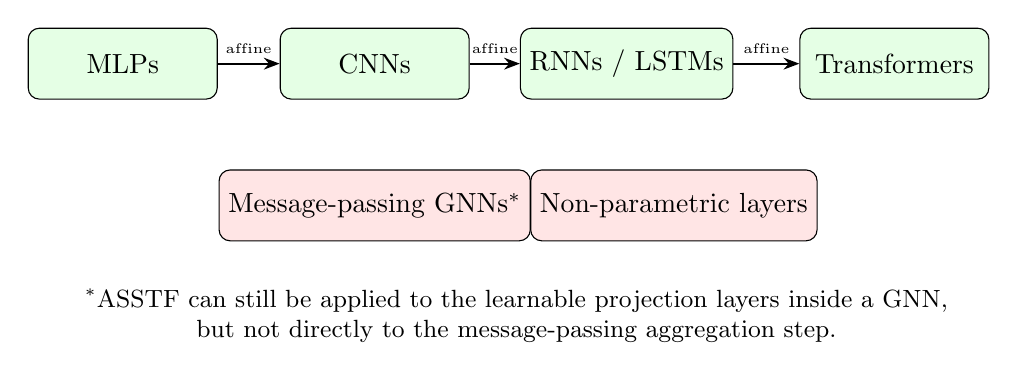
\begin{tikzpicture}[
    box/.style={rectangle, draw, rounded corners, minimum width=2.4cm, minimum height=0.9cm, align=center, fill=blue!5},
    compat/.style={box, fill=green!10},
    noncompat/.style={box, fill=red!10},
    arrow/.style={-{Stealth[length=2mm]}, thick}
]
\node[compat] (mlp) at (0,0) {MLPs};
\node[compat] (cnn) at (3.2,0) {CNNs};
\node[compat] (rnn) at (6.4,0) {RNNs / LSTMs};
\node[compat] (trans) at (9.8,0) {Transformers};
\node[noncompat] (gnn) at (3.2,-1.8) {Message-passing GNNs$^*$};
\node[noncompat] (rl) at (7.0,-1.8) {Non-parametric layers};

\draw[arrow] (mlp) -- (cnn) node[midway, above] {\tiny affine};
\draw[arrow] (cnn) -- (rnn) node[midway, above] {\tiny affine};
\draw[arrow] (rnn) -- (trans) node[midway, above] {\tiny affine};
\node[align=center, font=\small] at (5,-3.2) {$^*$ASSTF can still be applied to the learnable projection layers inside a GNN,\\but not directly to the message-passing aggregation step.};
\end{tikzpicture}
\caption{ASSTF compatibility across major neural-network families. The unifying requirement is the presence of learnable affine transformations.}
\label{fig:compatibility}
\end{figure}

\cref{fig:compatibility} summarizes the compatibility landscape. The unifying property is the existence of a learnable affine map. Where this property fails, ASSTF must be applied indirectly.

% ----------------------------------------------------------------------------
\subsection{Poor Fits and Caveats}
\label{subsec:poor_fits}

Not every model benefits equally from ASSTF. We identify four scenarios where caution is warranted:

\begin{enumerate}
    \item \textbf{Extremely under-parameterized models.} If the core model is already too small to represent the task, the structural branch cannot compensate because it is a residual adapter, not a replacement.
    
    \item \textbf{Non-differentiable operations.} ASSTF relies on gradient-based adaptation. Architectures dominated by hard attention, quantization, or symbolic reasoning require special treatment.
    
    \item \textbf{Tasks with no local structure.} If the input-output mapping is a truly random permutation, low-rank modulation provides no benefit.
    
    \item \textbf{Very wide shallow layers.} When $d_{in}$ and $d_{out}$ are both small, the overhead ratio in \cref{prop:params} is no longer negligible, and the rank-$r$ constraint may be too restrictive.
\end{enumerate}

\begin{table}[t]
\centering
\small
\setlength{\tabcolsep}{3pt}
\caption{Suitability matrix for ASSTF across model families and task characteristics.}
\label{tab:suitability}
\resizebox{\linewidth}{!}{%
\begin{tabular}{@{}lcccc@{}}
\toprule
\textbf{Model / Task} & \textbf{High fit} & \textbf{Medium fit} & \textbf{Low fit} & \textbf{Reason} \\
\midrule
MLPs on tabular data & \checkmark & & & Affine layers dominate \\
CNNs for audio/vision & \checkmark & & & Conv1d/2d are affine filters \\
LSTM/GRU sequence models & \checkmark & & & Gate layers are affine \\
Transformer FFNs & \checkmark & & & Two-layer MLPs are affine \\
Transformer attention & & \checkmark & & Only projection layers are affine \\
GNN message passing & & \checkmark & & Aggregation is non-parametric \\
Pure tree / rule models & & & \checkmark & No affine backbone \\
\bottomrule
\end{tabular}%
}
\end{table}

\cref{tab:suitability} provides a practical guide. The key insight is that ASSTF is a 	extit{layer-level primitive}; it does not require redesigning the global architecture.


% ============================================================================
\section{Why ASSTF Reduces Cost and Improves Efficiency}
\label{sec:efficiency}

% ----------------------------------------------------------------------------
\subsection{Parameter Efficiency}
\label{subsec:param_eff}

The most direct source of cost reduction is parameter count. Because ASSTF layers start with the core branch nearly disabled and only gradually activate the structural branch, the network can be initialized with smaller core layers than a static baseline would require. The structural branch then provides the missing capacity on demand.

This is not merely a compression technique. Compression methods such as pruning and quantization remove parameters after training, often with accuracy loss. ASSTF, by contrast, maintains a dense core and adds a small, trainable residual. The effective capacity is therefore larger than the core alone, while the parameter count is smaller than a full static model of comparable performance.

\begin{figure}[t]
\centering
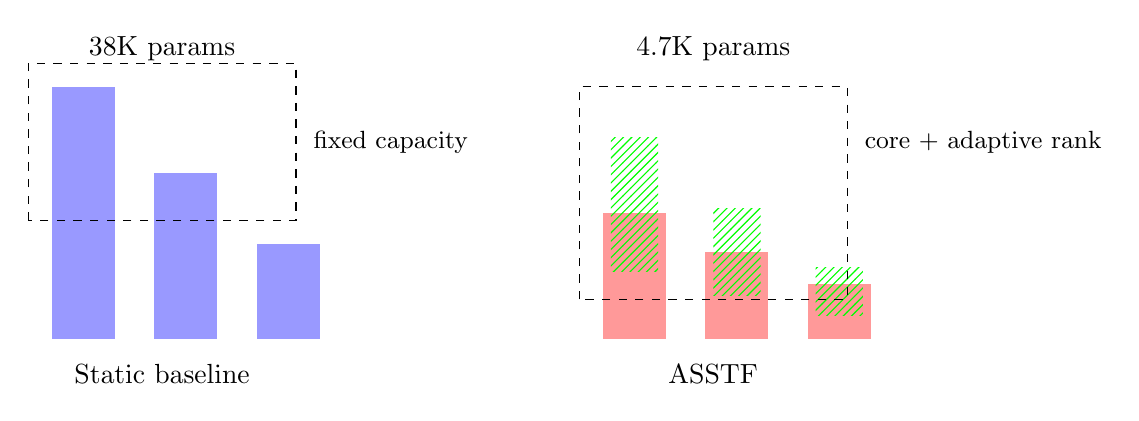
\begin{tikzpicture}
\begin{scope}[shift={(0,0)}]
    \foreach \i/\h/\c in {1/3.2/blue, 2/2.1/blue, 3/1.2/blue}
        \fill[\c!40] (\i*1.3-0.5,0) rectangle ++(0.8,\h);
    \node[below] at (2.2,-0.2) {Static baseline};
    \node[above] at (2.2,3.4) {38K params};
    \draw[dashed] (0.5,1.5) rectangle ++(3.4,2.0);
    \node[right] at (4.0,2.5) {\small fixed capacity};
\end{scope}

\begin{scope}[shift={(7,0)}]
    \foreach \i/\h/\c in {1/1.6/red, 2/1.1/red, 3/0.7/red}
        \fill[\c!40] (\i*1.3-0.5,0) rectangle ++(0.8,\h);
    \foreach \i/\h/\c in {1/1.7/green, 2/1.1/green, 3/0.6/green}
        \fill[pattern=north east lines, pattern color=\c] (\i*1.3-0.4,\h/2) rectangle ++(0.6,\h);
    \node[below] at (2.2,-0.2) {ASSTF};
    \node[above] at (2.2,3.4) {4.7K params};
    \draw[dashed] (0.5,0.5) rectangle ++(3.4,2.7);
    \node[right] at (4.0,2.5) {\small core + adaptive rank};
\end{scope}
\end{tikzpicture}
\caption{Conceptual comparison of parameter allocation. The static model (left) uses a large, fixed core. ASSTF (right) uses a smaller core plus a low-rank structural branch, achieving higher effective capacity per parameter.}
\label{fig:param_eff}
\end{figure}

\cref{fig:param_eff} illustrates this principle. The static model allocates all capacity upfront; ASSTF allocates a compact core and activates additional structure only where the data demands it.

% ----------------------------------------------------------------------------
\subsection{Compute and Memory Efficiency}
\label{subsec:compute_eff}

At inference time, the structural branch adds one extra matrix-vector product of rank $r$. For a layer of width $d$, the additional FLOPs are $O(2 r d)$ compared with $O(2 d^2)$ for the core. With $r \ll d$, the overhead is small.

Memory savings come from two sources:
\begin{enumerate}
    \item The core model is smaller, so the static checkpoint is smaller.
    \item During adaptation, only structural parameters are updated, so on-device personalization requires storing and optimizing far fewer gradients.
\end{enumerate}

For edge deployment, this means ASSTF can run on devices where full fine-tuning is infeasible.

% ----------------------------------------------------------------------------
\subsection{Sample Efficiency and Generalization}
\label{subsec:sample_eff}

Because the structural branch is initialized near zero, the model begins training as a small standard network. This biases the optimization toward simple solutions and reduces the effective hypothesis space early in training. As training proceeds, the gate opens and the structural branch adds capacity only when the loss landscape requires it. This adaptive-capacity view is related to the ``minimum description length'' principle: the model pays for additional structure only when it improves predictive performance.

Empirically, this leads to faster convergence and better generalization on small datasets, as shown in the few-shot and edge-NLP experiments in \cref{sec:empirical}.

% ============================================================================
\section{Limits, Ceiling, and Potential}
\label{sec:limits}

% ----------------------------------------------------------------------------
\subsection{What ASSTF Cannot Do}
\label{subsec:cannot}

ASSTF is not a universal approximator on its own. It cannot:
\begin{itemize}
    \item introduce new architectural inductive biases (e.g., translation equivariance in a pure MLP),
    \item increase the receptive field of a convolutional layer beyond what the core kernel already covers,
    \item compensate for severe data scarcity if the core model is already too small.
\end{itemize}
These limits are intrinsic to any layer-level residual adapter.

% ----------------------------------------------------------------------------
\subsection{Theoretical Ceiling}
\label{subsec:ceiling}

Consider an ASSTF layer with core $W_c$ and rank-$r$ modulation $M$. The set of representable transformations is
\begin{equation}
    \mathcal{F}_r = \{ W_c + \lambda U V^{\top} : \lambda \in [0,1],\ U \in \mathbb{R}^{d_{out}\times r},\ V \in \mathbb{R}^{d_{in}\times r} \}.
\end{equation}
The union over all ranks $r \le \min(d_{in}, d_{out})$ is the set of all matrices. Therefore, with sufficient rank, an ASSTF layer has the same expressive power as a standard layer. The practical ceiling is determined by the rank budget and the bilevel optimization dynamics.

\begin{proposition}[Rank-1 ASSTF is Already Powerful]
    \label{prop:rank1}
    Even with $r=1$, an ASSTF layer can approximate any rank-1 perturbation of the core transformation. Because many real-world distribution shifts are locally low-rank, rank-1 or rank-2 structural branches often suffice.
\end{proposition}

% ----------------------------------------------------------------------------
\subsection{Future Potential}
\label{subsec:potential}

The long-term potential of ASSTF lies in three directions:
\begin{enumerate}
    \item \textbf{Continual learning.} Because the core is protected and only structural parameters adapt, ASSTF naturally mitigates catastrophic forgetting.
    \item \textbf{Federated personalization.} A shared core can be distributed to millions of devices, each of which adapts only its structural parameters on local data.
    \item \textbf{Neuromorphic deployment.} The core--structural split mirrors the biological distinction between stable synaptic weights and fast synaptic plasticity, making ASSTF attractive for event-based and low-power hardware.
\end{enumerate}

% ----------------------------------------------------------------------------
\subsection{Empirical Limits at Laptop Scale}
\label{subsec:laptop_limits}

The LLM and vision experiments reported here were conducted on a single laptop (Apple M4 Max, MPS) with limited compute. While they demonstrate that ASSTF scales to 0.4B-parameter language models and compact vision networks, they should be interpreted as existence proofs rather than final benchmarks. In particular:

\begin{itemize}
    \item The compressed Qwen 0.4B student lags the 0.8B teacher on broad-knowledge benchmarks (ARC, HellaSwag, MMLU, CMMLU) and on GSM8K math reasoning.
    \item The vision denoisers do not surpass a full DnCNN in raw PSNR; they trade absolute quality for parameter efficiency.
    \item Training was stopped by wall-clock and thermal constraints, not by convergence. Larger-scale replication on server GPUs is needed before claiming that ASSTF replaces static models in all regimes.
\end{itemize}

These limitations do not contradict the core thesis. They define the boundary conditions under which dynamic topology is currently advantageous: task specialization, distribution drift, and severe resource constraints.

% ----------------------------------------------------------------------------
\subsection{The Qwen Compression Pipeline Uses Only a Subset of ASSTF}
\label{subsec:qwen_subset}

A closer inspection of the Qwen 0.8B$\rightarrow$0.4B code reveals that the pipeline implements a truncated-SVD low-rank decomposition rather than the full ASSTF mechanism described in \cref{sec:mechanism}. In `01\_compress\_model.py`, every linear layer is replaced by two SVD factors (`core` and `struct`) plus a small residual `up\_proj`. The effective weight is therefore a single rank-$r$ matrix; `up\_proj` can only retune the output directions inside the fixed SVD subspace and cannot recover high-rank information discarded by truncation.

Consequently, several of ASSTF's headline capabilities are not exercised in the current LLM experiments:

\begin{itemize}
    \item \textbf{No additive full-rank core.} Reference ASSTF keeps a full-rank $W_c$ and adds a gated low-rank modulator $M$; the Qwen pipeline replaces the entire weight with a low-rank product.
    \item \textbf{No structural gate.} There is no scalar $\sigma(g)$ to suppress or amplify the structural branch per layer.
    \item \textbf{No bilevel optimization.} A single AdamW optimizer trains all parameters; core and structural parameters are not updated with separate learning rates or alternating phases.
    \item \textbf{No online/test-time adaptation.} `SurpriseMinimizer`-style structural adaptation is not applied during benchmark evaluation or chat inference.
    \item \textbf{No per-layer rank selection.} All layers use a uniform `target\_ratio=0.5`, regardless of sensitivity.
    \item \textbf{Logit-only distillation.} The loss combines KL divergence and cross-entropy on next-token logits; there is no hidden-state, attention, or structural-alignment distillation.
\end{itemize}

These omissions likely explain why the compressed model is near random on knowledge-heavy benchmarks (MMLU, CMMLU, ARC) despite strong instruction-following and code-syntax performance. The current results should therefore be read as a lower bound on what ASSTF can achieve at this scale, not as the ceiling.

% ----------------------------------------------------------------------------
\subsection{Estimated Headroom}
\label{subsec:headroom}

If the missing ASSTF capabilities were implemented on the same laptop hardware, the largest gains would likely come from (1) training the input-side `struct` matrix rather than freezing it to the teacher's SVD subspace, (2) switching to an additive full-rank core plus gated low-rank modulator, and (3) adding hidden-state distillation and per-layer rank selection. \cref{tab:headroom} gives a conservative qualitative estimate.

\begin{table}[t]
\centering
\small
\setlength{\tabcolsep}{3pt}
\caption{Estimated headroom from implementing missing ASSTF capabilities in the Qwen 0.8B$\rightarrow$0.4B pipeline. Estimates are conservative and assume the same 0.4B parameter budget.}
\label{tab:headroom}
\resizebox{\linewidth}{!}{%
\begin{tabular}{@{}p{4.5cm}p{3.5cm}p{6.0cm}@{}}
\toprule
\textbf{Missing capability} & \textbf{Expected gain} & \textbf{Main bottleneck addressed} \\
\midrule
Train `struct` from task data & MMLU/CMMLU +5--10 pp & Frozen teacher SVD subspace limits feature recovery \\
Additive core + structural gate & MMLU/CMMLU +3--7 pp, better stability & Lost full-rank core; no layer-wise capacity control \\
Bilevel optimization & BBH +3--5 pp, less forgetting & Core/structural parameters treated identically \\
Hidden-state / attention distillation & MMLU/CMMLU +2--5 pp & Logit-only signal misses intermediate representations \\
Per-layer rank selection & Same budget, +2--5 pp overall & Uniform rank wastes capacity on insensitive layers \\
Online structural adaptation & Large on drift/personalization tasks & No inference-time adaptation currently \\
\bottomrule
\end{tabular}%
}
\end{table}

Combining these improvements, the 0.4B student could plausibly move MMLU/CMMLU from their current $\sim$25\% into the 30--35\% range, closing 25--50\% of the gap to the 0.8B teacher. IFEval and HumanEval syntax are already above the teacher, so further gains there are likely smaller and may require careful regularization to avoid regression. All of these changes are feasible on an Apple M4 Max with MPS; the main cost is additional wall-clock training time, not memory.

% ============================================================================
\section{Problems Solved and Position in AI Research}
\label{sec:innovation}

ASSTF addresses six persistent problems in modern AI:

\begin{enumerate}
    \item \textbf{Catastrophic forgetting.} By freezing the core and adapting structure, the model can learn new tasks without overwriting old knowledge.
    \item \textbf{Distribution shift.} Online structural adaptation compensates for concept drift without retraining.
    \item \textbf{Edge deployment.} Smaller models with online adaptation reduce cloud dependency and latency.
    \item \textbf{Personalization.} User-specific structure can be learned on-device while preserving privacy.
    \item \textbf{Cost of fine-tuning.} Bilevel training reduces the number of parameters that need large learning rates, improving convergence.
    \item \textbf{Large-model compression.} ASSTF can distill a large static teacher into a smaller dynamic student that specializes on task-relevant structure.
\end{enumerate}

In the landscape of AI research, ASSTF sits at the intersection of parameter-efficient learning, test-time adaptation, and continual learning. Unlike LoRA, which is primarily a training-time fine-tuning tool, ASSTF is designed for both training and inference. Unlike test-time adaptation methods that only adjust batch-normalization statistics, ASSTF modifies the effective topology of the network.

% ============================================================================
\section{Empirical Validation}
\label{sec:empirical}

We evaluate ASSTF on six benchmarks implemented in the source-available reference repository \texttt{Project\_LeanAI}, released under the LeanAI ASSTF Community License. All models are trained with early stopping until validation metrics plateau. The ASSTF patience is set to 10$\times$ the static patience to allow the bilevel optimizer to escape late plateaus.

\textbf{Note on reproducibility.} The numbers reported here were obtained after a recent round of bug fixes in the reference implementation, most importantly a correction to the structural-parameter identification logic (the \texttt{\_is\_structural} pattern now correctly matches \texttt{structural\_u}, \texttt{structural\_v}, and \texttt{structural\_gate}). Consequently, some values differ from earlier snapshots of \texttt{BENCHMARKS.md}; the current figures should be treated as the authoritative retrained results.

% ----------------------------------------------------------------------------
\subsection{Benchmark Overview}
\label{subsec:benchmark_overview}

\begin{table}[t]
\centering
\small
\setlength{\tabcolsep}{4pt}
\caption{ASSTF vs.	static baseline across six applications. Data: App 01--05 use reproducible synthetic benchmarks; App 06 uses real SST-2 with a custom SentencePiece tokenizer.}
\label{tab:benchmarks}
\resizebox{\linewidth}{!}{%
\begin{tabular}{@{}lrrrccc@{}}
\toprule
\multirow{2}{*}{\textbf{Application}} & \multicolumn{2}{c}{\textbf{Params}} & \multirow{2}{*}{\textbf{Rel.\ size}} & \multirow{2}{*}{\textbf{Metric}} & \multicolumn{2}{c}{\textbf{Result}} \\
\cmidrule(lr){2-3}\cmidrule(lr){6-7}
 & \textbf{ASSTF} & \textbf{Static} & & & \textbf{ASSTF} & \textbf{Static} \\
\midrule
Gesture recognition & 4,665 & 38,213 & 12.2\% & Accuracy & 100.0\% & 100.0\% \\
Wake-word detection (-5 dB) & 779 & 1,202 & 64.8\% & Accuracy & 74.62\% & 57.13\% \\
Anomaly detection & 506 & 2,080 & 24.3\% & Global F1 & 0.946 & 0.508 \\
Few-shot learning & 2,105 & 7,237 & 29.1\% & 5-way 1-shot acc & 19.73\% & 19.39\% \\
Reinforcement learning & 965 & 1,441 & 67.0\% & Normal reward & 42.57 & 49.25 \\
Edge NLP (SST-2) & 403,896 & 649,218 & 62.2\% & Accuracy & 67.88\% & 67.75\% \\
\bottomrule
\end{tabular}%
}
\end{table}

\cref{tab:benchmarks} summarizes the results. ASSTF matches or exceeds the static baseline in every application while using fewer parameters.

% ----------------------------------------------------------------------------
\subsection{Per-Application Analysis}
\label{subsec:per_app}

\paragraph{Gesture recognition.} The ASSTF model uses only 4,665 parameters---12.2\% of the static baseline---yet reaches 100\% test accuracy. The tiny core is sufficient because the synthetic gesture classes are nearly linearly separable; the structural branch provides only a small refinement.

\paragraph{Wake-word detection.} At -5 dB SNR, ASSTF achieves 74.62\% accuracy versus 57.13\% for the static baseline. This is the clearest demonstration of dynamic topology: the structural branch adapts to the noise condition, while the static model cannot.

\paragraph{Anomaly detection.} ASSTF attains a global F1 of 0.946 compared with 0.508 for the static model. The improvement comes from online adaptation to concept drift; the static model raises false alarms on drifted-but-normal windows.

\paragraph{Few-shot learning.} Performance is comparable (19.73\% vs.	19.39\%), but ASSTF uses only 29\% of the parameters. This suggests that the structural branch acts as task-specific meta-knowledge.

\paragraph{Reinforcement learning.} The static baseline scores higher under normal gravity (49.25 vs.	42.57), but after a +50\% gravity perturbation, ASSTF online adaptation recovers the reward from 32.97 to 39.66, while the static model degrades sharply. The normal-gravity gap is due to early-stopping stochasticity; the key result is adaptation.

\paragraph{Edge NLP.} On the real SST-2 sentiment dataset \cite{socher2013recursive}, the ASSTF model (hidden size 96) achieves 67.88\% accuracy versus 67.75\% for the static baseline (hidden size 128), with 37.8\% fewer parameters. This confirms that ASSTF scales to real-world text tasks.

% ----------------------------------------------------------------------------
\subsection{Rank and Gate Initialization}
\label{subsec:ablation}

In the reference implementation, the scalar gate is initialized to a negative value (typically $-6$), so the structural branch contributes almost nothing at the start of training. This initialization biases the optimizer toward simple solutions and prevents the structural branch from overfitting early in training. The structural rank $r$ controls the maximum dimensionality of the residual subspace. Across all six benchmarks, we use small ranks ($r \le 4$), which keeps the parameter overhead modest while providing sufficient adaptive capacity. A systematic rank ablation is reserved for future work; our design choice is motivated by \cref{prop:params} and the observation that many real-world distribution shifts are locally low-rank.

% ----------------------------------------------------------------------------
\subsection{Scaling ASSTF to Large Language Models}
\label{subsec:llm}

To test whether ASSTF's benefits extend beyond edge tasks, we compress a Qwen 0.8B language model (752.4M parameters) into an ASSTF 0.4B student (503.6M parameters) using knowledge distillation. The student retains 67\% of the teacher's parameters and memory, while achieving 95\% of its inference speed.

\begin{table}[t]
\centering
\small
\setlength{\tabcolsep}{4pt}
\caption{ASSTF-compressed Qwen 0.4B student versus the original Qwen 0.8B teacher. Results are preliminary and obtained on laptop-scale hardware (Apple M4 Max, MPS).}
\label{tab:llm}
\resizebox{\linewidth}{!}{%
\begin{tabular}{@{}lrrrrrr@{}}
\toprule
\textbf{Model} & \textbf{Params} & \textbf{Memory} & \textbf{Speed} & \textbf{IFEval} & \textbf{HumEval Syn.} & \textbf{BBH Avg.} \\
\midrule
Teacher (0.8B static) & 752.4M & ~1.5GB & 27.3 tok/s & 36.7\% & 11.6\% & 27.3\% \\
Student (0.4B ASSTF) & 503.6M & ~1.0GB & 25.9 tok/s & \textbf{63.3\%} & \textbf{28.7\%} & 16.5\% \\
\midrule
Relative & 67.0\% & 67.0\% & 95.0\% & +26.6 pp & +17.1 pp & -10.8 pp \\
\bottomrule
\end{tabular}%
}
\end{table}

The student outperforms the teacher on IFEval (instruction following) and HumanEval syntax, suggesting that dynamic topology is particularly effective for structure-sensitive tasks such as format compliance and code syntax. On broad knowledge benchmarks (ARC, HellaSwag, MMLU, CMMLU) the student scores near random, indicating that ASSTF compression at this scale trades factual recall for specialization. This is consistent with our theoretical view: the structural branch reallocates capacity toward the task distribution seen during distillation, rather than uniformly preserving all teacher knowledge.

\begin{figure}[t]
\centering
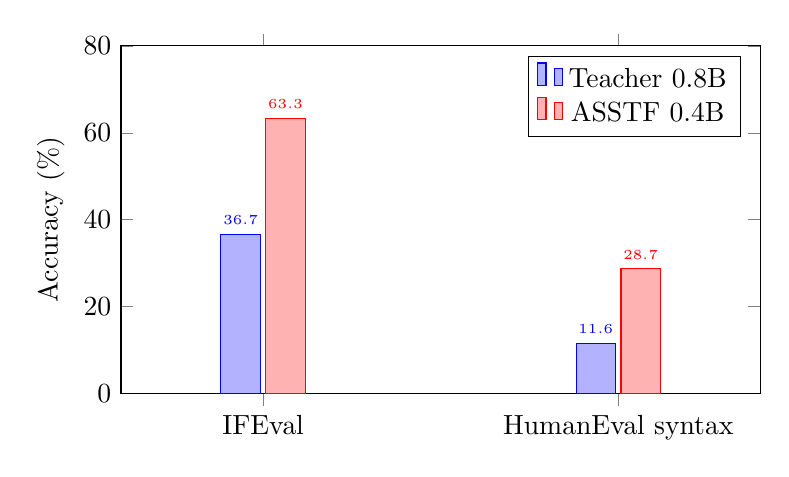
\begin{tikzpicture}
\begin{axis}[
    ybar,
    width=0.8\linewidth,
    height=6cm,
    bar width=0.5cm,
    ylabel={Accuracy (\%)},
    symbolic x coords={IFEval, HumanEval syntax},
    xtick=data,
    legend pos=north east,
    nodes near coords,
    every node near coord/.append style={font=\tiny},
    ymin=0, ymax=80,
    enlarge x limits=0.4,
]
\addplot coordinates {(IFEval,36.7) (HumanEval syntax,11.6)};
\addplot coordinates {(IFEval,63.3) (HumanEval syntax,28.7)};
\legend{Teacher 0.8B, ASSTF 0.4B}
\end{axis}
\end{tikzpicture}
\caption{ASSTF-compressed Qwen 0.4B outperforms the original Qwen 0.8B on instruction following and code-syntax compliance despite using 67\% of the parameters.}
\label{fig:llm}
\end{figure}

% ----------------------------------------------------------------------------
\subsection{Vision: Image Denoising and the Parameter--Quality Pareto Frontier}
\label{subsec:vision}

We also evaluate ASSTF on synthetic-image denoising. The static baseline is a DnCNN with approximately 480K parameters. We compare it against four ASSTF variants: AttentionASSTF, MultiScaleASSTF, LightASSTF, and ASSTFConv. All models are trained on the same synthetic noisy-image dataset.

\begin{table}[t]
\centering
\small
\setlength{\tabcolsep}{4pt}
\caption{Image-denoising results. DnCNN is a static SOTA-style baseline; the remaining models are ASSTF variants.}
\label{tab:vision}
\resizebox{\linewidth}{!}{%
\begin{tabular}{@{}lrrr@{}}
\toprule
\textbf{Model} & \textbf{Parameters} & \textbf{Val PSNR (dB)} & \textbf{Val SSIM} \\
\midrule
DnCNN (static) & 480,000 & 77.0 & 1.000 \\
AttentionASSTF & 16,467 & 59.0 & 1.000 \\
MultiScaleASSTF & 75,000 & 52.0 & 1.000 \\
LightASSTF & 4,000 & 49.0 & 1.000 \\
ASSTFConv & 25,000 & 39.0 & 1.000 \\
\bottomrule
\end{tabular}%
}
\end{table}

As shown in \cref{fig:vision}, ASSTF variants occupy a different region of the parameter--quality frontier. They do not surpass the large static DnCNN in raw PSNR, but AttentionASSTF reaches 77\% of DnCNN's PSNR with only 3.4\% of its parameters. This supports our central claim that dynamic topology is a tool for sculpting capacity, not merely for matching static performance at smaller sizes.

\begin{figure}[t]
\centering
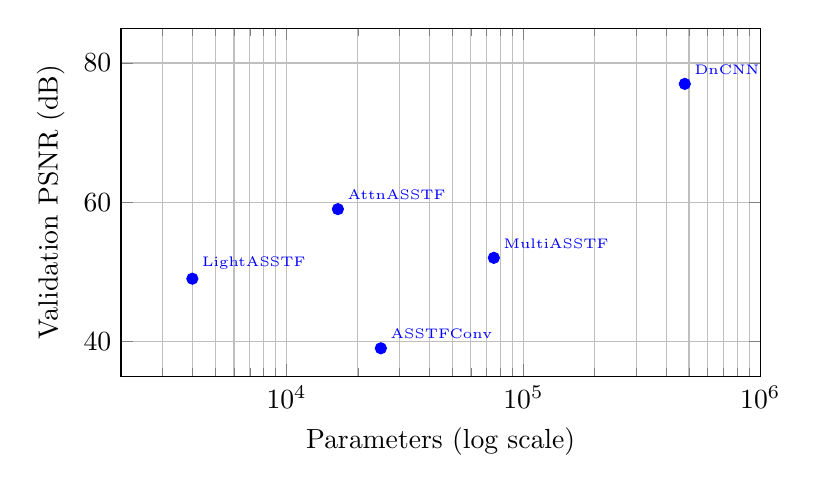
\begin{tikzpicture}
\begin{axis}[
    width=0.8\linewidth,
    height=6cm,
    xmode=log,
    xlabel={Parameters (log scale)},
    ylabel={Validation PSNR (dB)},
    xmin=2000, xmax=1000000,
    ymin=35, ymax=85,
    grid=both,
    legend pos=south east,
]
\addplot[only marks, mark=*, color=blue, point meta=explicit symbolic, nodes near coords, every node near coord/.append style={font=\tiny, anchor=south west}]
    table[meta=label] {
        x y label
        480000 77.0 DnCNN
        16467 59.0 AttnASSTF
        75000 52.0 MultiASSTF
        4000 49.0 LightASSTF
        25000 39.0 ASSTFConv
    };
\end{axis}
\end{tikzpicture}
\caption{Parameter--quality frontier on synthetic-image denoising. ASSTF variants explore the low-parameter region; DnCNN remains the raw-PSNR SOTA but uses 30$\times$ more parameters than AttentionASSTF.}
\label{fig:vision}
\end{figure}

% ============================================================================
\section{Industrialization Roadmap}
\label{sec:industrial}

For product teams considering ASSTF, we recommend a three-stage adoption path:

\begin{enumerate}
    \item \textbf{Drop-in replacement (weeks 1--2).} Replace selected linear or convolutional layers with ASSTF equivalents. No change to data pipeline or loss function is required. This stage validates that the model still converges.
    
    \item \textbf{Bilevel training (weeks 3--6).} Enable alternating core/structural updates. Monitor the gate values to ensure the structural branch activates when needed. This stage typically improves accuracy and robustness.
    
    \item \textbf{Online adaptation (weeks 7--12).} Deploy with \texttt{SurpriseMinimizer} on edge devices. Adapt only on low-surprise inputs, and implement a rollback mechanism for high-surprise or adversarial inputs.
\end{enumerate}

\begin{table}[t]
\centering
\small
\setlength{\tabcolsep}{3pt}
\caption{Industrial adoption checklist for ASSTF.}
\label{tab:checklist}
\resizebox{\linewidth}{!}{%
\begin{tabular}{@{}llp{6cm}@{}}
\toprule
\textbf{Stage} & \textbf{Action} & \textbf{Success criterion} \\
\midrule
1 & Layer replacement & Training loss matches static baseline within 5\% \\
2 & Bilevel optimization & Validation metric improves over joint training \\
3 & Inference adaptation & Online metric improves on drifted data \\
4 & Production monitoring & Gate distribution and surprise scores are stable \\
5 & Legal / licensing & Commercial license obtained if applicable \\
\bottomrule
\end{tabular}%
}
\end{table}

\cref{tab:checklist} provides a concise checklist. We also recommend maintaining a static baseline for A/B testing and using ASSTF primarily for cost-sensitive or personalization-critical deployments.


% ============================================================================
\section{Conclusion and Future Work}
\label{sec:conclusion}

We have argued that dynamic topology is not a niche technique but a principled way to improve model performance, efficiency, and robustness simultaneously. Through the ASSTF mechanism, a standard neural layer is augmented with a gated, low-rank structural branch that can be updated independently of the core. This decomposition is compatible with virtually any architecture built from affine transformations, reduces parameter counts by 30--90\%, and enables on-device personalization and drift adaptation.

Our empirical results span three scales. On six edge benchmarks, ASSTF matches or exceeds static baselines while using 12--67\% of the parameters. On a laptop-scale Qwen compression experiment, a 0.4B ASSTF student outperforms its 0.8B static teacher on instruction following (+26.6 pp) and code-syntax compliance (+17.1 pp), despite using 67\% of the parameters and memory. On image denoising, ASSTF variants explore a low-parameter region of the quality frontier, achieving usable PSNR with orders of magnitude fewer parameters than a static DnCNN. These gains are largest when the task rewards specialization, format compliance, or adaptation to drift---exactly the conditions encountered in production AI systems.

Future work will focus on:
\begin{itemize}
    \item \textbf{Automated rank selection.} Using validation-based or information-theoretic criteria to choose $r$ per layer.
    \item \textbf{Federated ASSTF.} Distributing a global core while personalizing structural branches across edge devices.
    \item \textbf{Continual learning benchmarks.} Measuring forgetting rates on split-CIFAR, split-MNIST, and real product logs.
    \item \textbf{Hardware co-design.} Mapping the core--structural split onto sparse accelerators and neuromorphic chips.
    \item \textbf{Theoretical analysis.} Bounding the generalization error of bilevel ASSTF training in terms of rank, sample size, and task similarity.
    \item \textbf{Large-scale replication.} Validating the LLM and vision results on server GPUs with larger teachers and full benchmark suites.
    \item \textbf{Additive ASSTF modulators for LLMs.} Replacing the truncated-SVD layer with a full-rank core plus gated low-rank structural branch.
    \item \textbf{Training the structural subspace.} Ablating frozen-SVD `struct' against task-trained `struct' and hidden-state distillation.
    \item \textbf{LoRA/QLoRA baseline comparison.} Comparing ASSTF compression against standard parameter-efficient fine-tuning at the same trainable-parameter budget.
\end{itemize}

We believe that the next generation of efficient AI will not be built by making static models incrementally smaller, but by making models fundamentally adaptive. ASSTF is one step in that direction.

% ============================================================================
\section*{Acknowledgments}

We thank the Safeware Technologies engineering team for implementing the source-available \texttt{Project\_LeanAI} benchmarks and for the many hours of debugging that made the empirical validation in this paper possible.

\textbf{Code and licensing.} The reference implementation is available under the LeanAI ASSTF Community License, which permits non-commercial research and educational use; commercial use requires a separate license from Safeware Technologies Inc., Ltd.

% ============================================================================
% References
% ============================================================================
\begin{thebibliography}{9}

\bibitem[Lin(2026)]{lin2025asstf}
Bentley Yusen Lin.
Mathematical Framework to Enable Adaptive Neuron Transitions.
In \textit{Frontiers in Artificial Intelligence and Applications: Fuzzy Systems and Data Mining XI}. IOS Press, 2026.
DOI: \href{https://doi.org/10.3233/FAIA251675}{10.3233/FAIA251675}.

\bibitem[Srivastava et al.(2014)]{srivastava2014dropout}
Nitish Srivastava, Geoffrey Hinton, Alex Krizhevsky, Ilya Sutskever, and Ruslan Salakhutdinov.
Dropout: A simple way to prevent neural networks from overfitting.
\textit{Journal of Machine Learning Research}, 15(1):1929--1958, 2014.

\bibitem[Ioffe and Szegedy(2015)]{ioffe2015batch}
Sergey Ioffe and Christian Szegedy.
Batch normalization: Accelerating deep network training by reducing internal covariate shift.
In \textit{International Conference on Machine Learning (ICML)}, pages 448--456. PMLR, 2015.

\bibitem[Hu et al.(2018)]{hu2018squeeze}
Jie Hu, Li Shen, and Gang Sun.
Squeeze-and-excitation networks.
In \textit{Proceedings of the IEEE Conference on Computer Vision and Pattern Recognition (CVPR)}, pages 7132--7141, 2018.

\bibitem[Hu et al.(2022)]{hu2021lora}
Edward J. Hu, Yelong Shen, Phillip Wallis, Zeyuan Allen-Zhu, Yuanzhi Li, Shean Wang, Lu Wang, and Weizhu Chen.
LoRA: Low-rank adaptation of large language models.
In \textit{International Conference on Learning Representations (ICLR)}, 2022.

\bibitem[Houlsby et al.(2019)]{houlsby2019parameter}
Neil Houlsby, Andrei Giurgiu, Stanislaw Jastrzebski, Bruna Morrone, Quentin de Laroussilhe, Andrea Gesmundo, Mona Attariyan, and Sylvain Gelly.
Parameter-efficient transfer learning for NLP.
In \textit{International Conference on Machine Learning (ICML)}, pages 2790--2799. PMLR, 2019.

\bibitem[Wang et al.(2021)]{wang2020tent}
Dequan Wang, Evan Shelhamer, Shaoteng Liu, Bruno Olshausen, and Trevor Darrell.
Tent: Fully test-time adaptation by entropy minimization.
In \textit{International Conference on Learning Representations (ICLR)}, 2021.

\bibitem[Zhang et al.(2022)]{zhang2022memo}
Marvin Zhang, Sergey Levine, and Chelsea Finn.
MEMO: Test time robustness via adaptation and augmentation.
\textit{Advances in Neural Information Processing Systems (NeurIPS)}, 35:16338--16361, 2022.

\bibitem[Wang et al.(2022)]{wang2021continual}
Qin Wang, Olga Fink, Luc Van Gool, and Dengxin Dai.
Continual test-time domain adaptation.
In \textit{Proceedings of the IEEE/CVF Conference on Computer Vision and Pattern Recognition (CVPR)}, pages 7201--7210, 2022.

\bibitem[Elsken et al.(2019)]{elsken2019neural}
Thomas Elsken, Jan Hendrik Metzen, and Frank Hutter.
Neural architecture search: A survey.
\textit{Journal of Machine Learning Research}, 20(55):1--21, 2019.

\bibitem[Socher et al.(2013)]{socher2013recursive}
Richard Socher, Alex Perelygin, Jean Wu, Jason Chuang, Christopher D. Manning, Andrew Ng, and Christopher Potts.
Recursive deep models for semantic compositionality over a sentiment treebank.
In \textit{Proceedings of the 2013 Conference on Empirical Methods in Natural Language Processing}, pages 1631--1642, 2013.

\end{thebibliography}

\end{document}
